The crowdsourcing video annotation approach presented in this paper follows three steps: Preparation, Annotation, and Presentation. 

The preparation step describes how a complex annotation task can be divided into simple microtasks, in addition is presented a workflow for the activities required before the annotation step, such as to define what should be annotated and the annotation types, as well as to design the microtasks and the simple annotation tools to execute them. In the annotation step the annotation microtasks are performed by crowd workes, that are the contributors for the process. This step follows a workflow in which each microtask is followed by a specific aggregation method that generates a result, so that the output from a task feeds the next one. The presentation step displays the outcome delivered by the annotation step, also at this point all partial results are available to be used in other applications. The approach introduced also allows the development of expansive video annotation systems in which it is easily possible to add new microtasks to improve its result or generate new results. 

These steps contains specific activities, and are executed sequentially how can be seen in Figure~\ref{process}.

\begin{figure}[h]
	\centerline{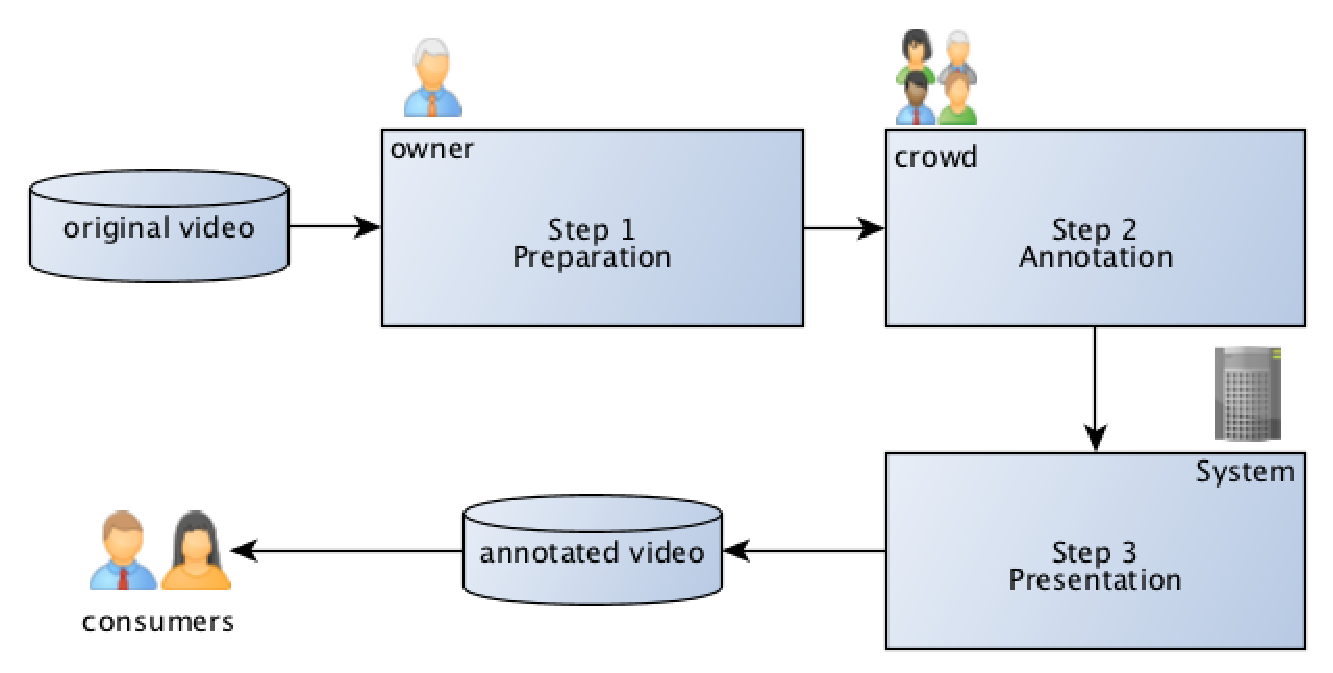
\includegraphics[scale=0.4] {figure/process}}
	\caption{Process workflow}
	\label{process}
\end{figure}

\textbf{Preparation:} all activities involved in this step are performed by the owner, who started the video annotation process. At this step is determined what must be annotated, also how they should be annotated. In this way the owner must determine:
\begin{enumerate}
\item What kinds of point of interest should be annotated.\\Ex: events, objects, subjects, issues.
\item What annotation type will be used for each of these kinds.\\Ex: free write, item select, button click, image upload.
\item What data type will be collected for each annotation type.\\Ex: plain text, location, image, video.
\end{enumerate}

To illustrate this point, the example of the football(soccer) match annotation will be recalled. In a football(soccer) match video the kinds of point of interest correspond to events such as goals, cards and faults. For each point of interest observed it should be collected its kind, and the instant when this event happened. The annotation type to be used on the annotation tool can be a set of icons related to each event. Finally, the data type collected in this case may be plain text that contains the kind of event identified and the instant it happened \cite{santos2007estrategia}.

Also it is important to provide explanations or guidelines that can instruct the workers about how execute the microtasks. An additional activity on the Preparation step is determine what section of the video should be send by each worker, this division can be made by duration (ex: send a 5 seconds segment to each worker), or using contextual criteria such as to send to each user a segment that contains a single dialog. The activities sequence for this step can be observed on Figure~\ref{preparation}.

\begin{figure}[h]
	\centerline{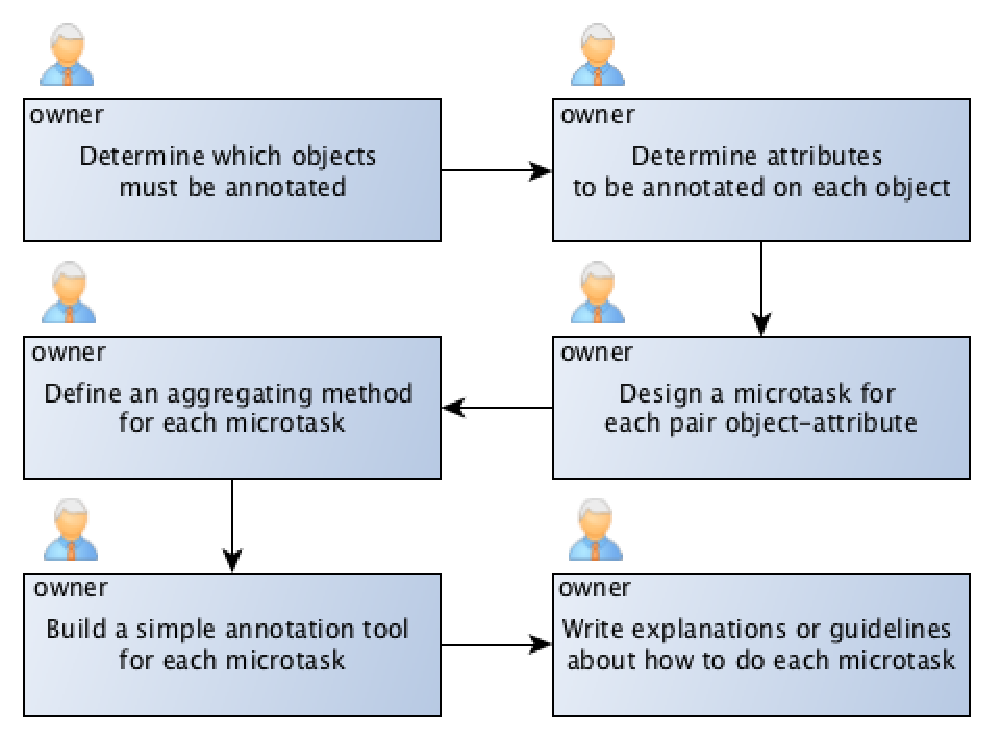
\includegraphics[scale=0.4] {figure/preparation}}
	\caption{Preparation step}
	\label{preparation}
\end{figure}


\textbf{Annotation:} an essential aspect for this step is to determine the microtasks' workflow, so the output from a task is taken as input by the next one, generating a final outcome at the end of the last microtask. This cascade workflow is illustrated in Figure~\ref{cascading}. It is important to notice that each task cell in composed by two activities, the microtask in self and the aggregation method, that generates the output from the obtained contributions. In this way, the output from the last task cell is the final outcome provided by the system.

\begin{figure}[h]
	\centerline{\includegraphics[scale=0.25] {figure/cascading}}
	\caption{Annotation step for N microtasks}
	\label{cascading}
\end{figure}

\textbf{Presentation:} at this step is generated an annotated video including the original video and the final outcome from the previous step. Other activities that can be proceeded at this step is to generate, or to render, media items selected from the crowd annotations, as well as aggregate these items over the videos to compose a multimedia presentation.

\begin{figure}[h]
	\centerline{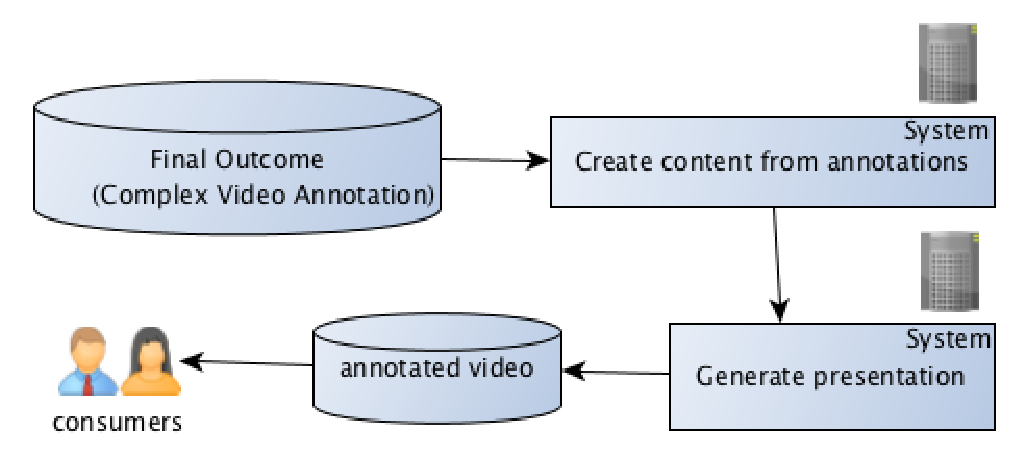
\includegraphics[scale=0.5] {figure/presentation}}
	\caption{Presentation step}
	\label{presentation}
\end{figure}








